\documentclass[a4paper,onecolumn,11pt]{article}
%%%%
\renewcommand{\familydefault}{\sfdefault}%
%%%

%Packages%%%%%%%%%%%%%%%%%%%%
\usepackage[margin=2cm]{geometry} %this assures 2cm margin on all sides
\usepackage{graphicx}% to include figures
\usepackage{array}%
\usepackage{hyperref}
\hypersetup{linkcolor=blue, pdftitle={Quantifying Software Quality through Data Change Validation}, pdfauthor={Dominic Roberts}, pdfsubject={Research Proposal Assignment -- January 2018}, pdfkeywords={software quality, software testing, mutation testing, genetic algorithms} }
%%%%%%%%%%%%%%%%%%%%%%%%%%%%%%%%%%%%%%%%%%%%%%%%%%%%%%%%%%%%%%%%%%%%%%%%%%%%%%%%%%%%%%%%%%%%%%%%%%%%%%%%%%%%%%%%%%%%%%%%%%%%%%%%%%%%%%%%%%%%%%%%%%%%%%%%%%%%%%%%%%%%%%%%%%
%%DOUBLE QUOTE and SINGLE QUOTE Commands%
\newcommand{\qq}[1]{\textquotedblleft#1\textquotedblright}%
\newcommand{\q}[1]{\textquoteleft#1\textquoteright}%
\pagenumbering{arabic}%
%\setcounter{page}{-1}%
\begin{document}
\title{\vspace{-2.5cm}Solving the NQueens problem with Genetic Algorithms seeded by lower dimension results}
\author{\textbf{Dominic Roberts}\\
\textbf{P17201056}\\
MSc Intelligent Systems, De Montfort University
}%
%%%%%%%%%%%%%%%%%%%%%%%%%%%%%%%%%%%%%%%%%%%%%%%%%%%%%%%%%%%%%%%%%%%%%%%%%%%%%%%%%%%%%%%%%%%%%%%%%%%%%%%%%%%%%%%%%%%%%%%%%%%%%%%%%%%%%%%%%%%%%%%%%%%%%%%%%%%%%%%%%%%%%%%%%%
% make the title area
\maketitle
\thispagestyle{empty}
%%%%%%%%%%%%%%%%%%%%%%%%%%%%%%%%%%%%%%%%%%%%%%%%%%%%%%%%%%%%%%%%%%%%%%%%%%%%%%%%%%%%%%%%%%%%%%%%%%%%%%%%%%%%%%%%%%%%%%%%%%%%%%%%%%%%%%%%%%%%%%%%%%%%%%%%%%%%%%%%%%%%%%%%%%

\section{Abstract}
The 8-Queens problem was devised by Max Bezzel in 1848 and consists of a challenge to place 8 Queens on a chess board such that none of the Queens are able to attack another Queen. The more general form of the problem is known as the N-Queens problem where N denotes the dimensions of the board and subsequent count of Queens. The problem is known to be NP-Complete \cite{Complexity}. There have been many different solutions found for the problem, the original solution was provided by Franz Nauck in 1850. It has been used as a benchmark for AI research due in part to it being an Np-Complete problem that is easy to explain to anyone with a basic understanding of Chess. Due to its popularity there have been numerous attempts to resolve the problems using Genetic Algorithms (GA) previously. However, this paper describes a technique that uses the outcomes from lower dimensional evaluations to seed the GA in order to massively improve the performance in searching for solutions in the given dimensions. By reusing previous successful solutions from a lower n-dimensionality it aims to show that there is a close correlation between the results from each dimension and that combinatorial problems like the N-Queens problem can be simplified by applying lower dimensional solutions to higher order problems.

\section{Introduction}
In the game of Chess the Queen is the only piece on the board that is permitted to move any number of spaces horizontally, vertically and diagonally. On a standard 8x8 board it can attack up to 21 different squares in a single move. In 1848 Max Bezzel proposed a puzzle for calculating a configuration whereby 8 Queens can be placed on a board without any two pieces being able to attach each other. This problem, known as the 8-Queens problem, has a more generic variant that imposes the same rules on boards of any topology such that the for N dimensions, there are NxN squares on the board and N Queens to be placed. Since the initial proposition of the puzzle there have been many different approaches to solving it. The first person to successfully find all 92 placements of the original 8x8 board was Pauls \cite{Pauls} in 1874. Work has continued since to resolve the solutions for higher dimensions, currently the maximum dimensions for which all solutions have been proven is 27, for which there are 234,907,967,154,122,528 solutions a result that took over a year of computing time to calculate\cite{27Queens}. This limitation is due to the enormous number of solutions at higher dimensionalitys. The possible combinations of a board layout is $N^{N}$ and so the possible valid permutations grows exponentially as the dimensions are increased. Table 1. lists a selection the number of permutations for the board layout.

\begin{table*}[h]
	\caption{Possible Permutation for Queen positions on a N Dimensional Chess board} % title of Table
	\begin{tabular}{l l} 
		\hline\\
		Dimensions & Combinations \\
		\hline\\
		8 & 16,777,216 \\ 
		9 & 387,420,489 \\
		10 & 10,000,000,000 \\
		15 & 437,893,890,380,859,375 \\
		20 & 104,857,600,000,000,000,000,000,000
	\end{tabular}
\end{table*}

The first implementation of a Genetic Algorithm (GA) to solve the problem was by Crawford \cite{Crawford} in 1994. Since this point a variety of Heuristic algorithms have been configured to resolve the problem \cite{AdvanceMutation} \cite{ACO} \cite{comparison} \cite{PSO}. Although the N-Queens puzzle is NP-Hard it is a very simple to describe to anyone familiar with the game of Chess. This has led to it becoming a benchmark problem for the development and testing of Heuristic solutions. Brute force approaches to solving the problem are effective at calculating the results for all combinations over the lower ranges of dimensions, but as the number of possible combinations increases, so the time required to evaluate all potential options becomes prohibitive.

This paper introduces a variation on the standard Genetic Algorithm. The technique developed seeds the initial search locations for the algorithm with result sets obtained from a lower dimension. Valid board configurations from a smaller board are enhanced with additional fields to boost the dimensions to the required size and then set as the initial genome location in new clusters of genomes. The rest of this paper is organised as follows the next section will give more detail of the N-Queens problem, this is followed by an overview of Genetic Algorithms and their implementations. An analysis of related works is then given to give additional context to the problem and existing research into the use of Heuristic algorithms to solve it. The subsequent section will detail the approach that has been developed in this paper and that is then followed by an analysis of the results obtained. Finally, the paper will discuss the outcomes and conclusions from the research and indicate a number of potential areas for further investigation.

\section{N Queens}
The N-Queens problems requires N Queens to be placed on an $NxN$ chess board such that no two Queens are able to attack each other. On an N dimensional board there are $N^{N}$ possible placements for the N Queens. However, as any Queen placed on the same column or row as another would immediately invalidate that combination. Thus the permutations can be reduced to !N configuration as each piece is restricted to a single piece per column and per row.

\begin{figure}[!htbp]
	\centering	
	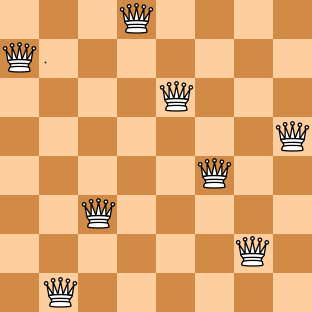
\includegraphics[width=6cm, height=6cm]{Valid8QueensSolution}
	\caption{An example of a valid 8 Queens solution where no 2 Queen placements are able to attack another Queen.}
\end{figure}
It can be seen from Figure 1 that as long as no two pieces are on the same Horizontal or Vertical as another then the only concern when resolving the problem is the diagonals. 

It is possible to determine valid results for all dimensions above 3. There are no possible solutions for N=2 or N=3. The following table gives the number of available solutions for a range of values for N. As the number of dimensions increases the possible solutions also increases for all values apart from 6 for which there are only 4 valid configurations. 

\begin{table*}[ht]
\begin{tabular}{|p{2cm}|p{6cm}|p{6cm}|} 
		\hline\\
		Dimensions & Solutions & Unique Solutions \\
		\hline\\
		4 & 2 & 1 \\ 
		5 & 10 & 2 \\
		6 & 4 & 1 \\
		7 & 40 & 6 \\
		8 & 92 & 12 \\
		9 & 352 & 46 \\
		10 & 724 & 92 \\
		15 & 2,279,184 & 285,053 \\
		20 & 39,029,188,884 & 4,878,666,808 \\
		25 & 2,207,893,435,808,350  & 275,986,683,743,434 \\
		26 & 22,317,699,616,364,000 & 2,789,712,466,510,280 \\
		\hline
	\end{tabular}
	\caption{The number of Solutions and Unique Solutions for a range of values for N}
\end{table*}

Table 1 gives the number of solutions along with the unique variants at each dimension. For every solution to the problem it is possible that there is also a rotational or reflected variant that could also be a valid configuration. By rotating the board through 90, 180 and 270 degrees or reflecting along the central X and Y axis of the board then further valid solutions can be found.

\begin{figure}[!htbp]
	\centering	
	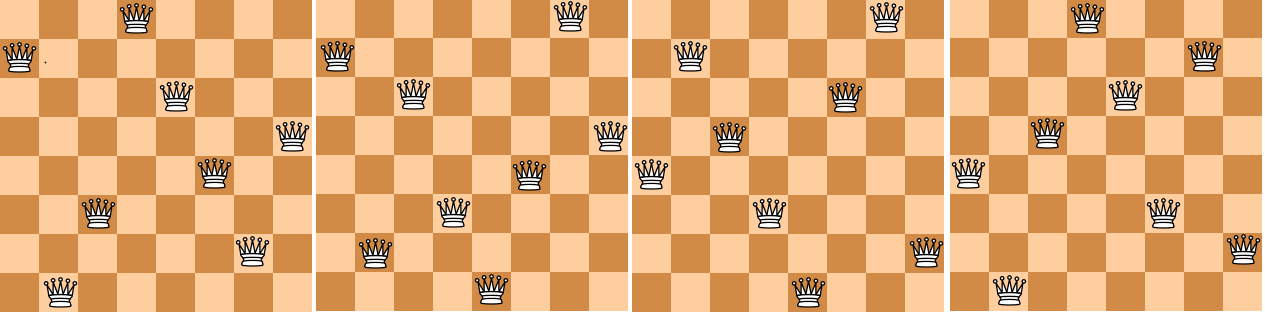
\includegraphics[width=16cm, height=4cm]{NQueensRotations}
	\caption{By rotating a configuration through 360 degrees further valid solutions can be derived.}
\end{figure}

\begin{figure}[!htbp]
	\centering	
	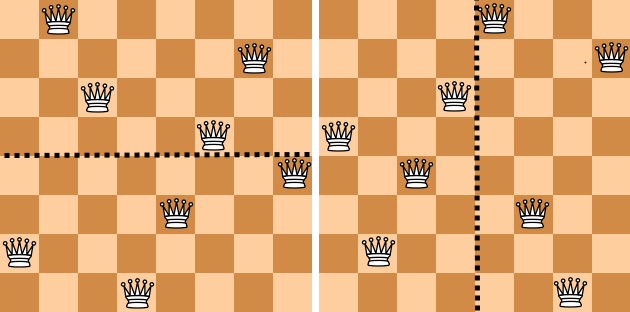
\includegraphics[width=8cm, height=4cm]{Valid8QueensReflected}
	\caption{By reflecting the layout along the X and Y axis other valid solutions can be derived.}
\end{figure}

The ability to locate up to an additional 5 solutions from an initial configuration improves the performance of a Search algorithm. Each time a new solution is found analysing each of the transformations can yield multiple valid layouts.

Although it is generally considered to be merely a mathematical puzzle there are numerous real world applications for solutions to the problem.


\section{Implementation}
\subsection{Genetic Algorithm}
The implemented genetic algorithm starts by generating clusters of genomes known as Demes \cite{Demes}. The Demes group genomes together around an initial starting location and on each iteration are modified in relation to the best performing Deme member. The size of each group is initiated from a starting parameter set that can be configured per run of the algorithm. Each genome in the Deme is instantiated with a starting location. Locations are defined as an integer array with each column in the array representing a row number for the location of the queen in that row. Each row can be assigned a single value as having multiple locations within the same column would immediately render the board combination invalid as multiple Queens would be in opposable positions. The Deme is generated and each genome is assigned to a mini tournament of 3 members taken randomly from the Deme. On each iteration the Deme members each calculate their current fitness value via the N-Queens fitness function. If this updated value is an improvement on the members previous best fitness, then the best value and location are updated to reflect this improvement. Each of the mini-tournaments within a Deme are then contested, the competitor with the best fitness, over the duration of the members lifetime and not just a single round, is retained for the next iteration. All losing members of the tournament are discarded. Through this process the population of each Deme is reduced by 2/3 on each iteration. These members are then replaced through a stochastic Cross-Over process where two parents are selected form the list of tournament winners.

\begin{thebibliography}{99.}

\bibitem {Complexity} Gent I.P., Jefferson C., Nightingale P. 	Complexity of n-Queens Completion Journal of Artificial Intelligence Research 59 (2017) 

\bibitem {Pauls} E. Pauls, Das Maximalproblem der Damen auf dem Schachbrete, Deutsche Schachzeitung. Organ fur das Gesammte Schachleben 29 (5) (1874) 129–134.

\bibitem {Crawford} Kelly D. Crawford, Solving n-Queen problem using genetic algorithms SAC '92 Proceedings of the 1992 ACM/SIGAPP symposium on Applied computing,pp:1039-1047,1994 

\bibitem {Demes} Nowostawski, Mariusz and Poli, Riccardo. (1999). Dynamic Demes Parallel Genetic Algorithm. 10.1109/KES.1999.820128. 

\bibitem{27Queens} https://github.com/preusser/q27

\bibitem{AdvanceMutation} V. Jain, J.S. Prasad, (2018) Solving N-queen Problem Using Genetic Algorithm by Advance Mutation Operator. International Journal of Electrical and Computer Engineering

\bibitem{ACO} Khan, Salabat. Bilal, Mohsin. Sharif, Muhammad. Sajid Abbas. Malik, Baig, Abdul. (2010). Solution of n-Queen problem using ACO. 1 - 5. 10.1109/INMIC.2009.5383157. 

\bibitem{comparison} Martinjak, Ivica. Golub, M. (2007). Comparison of Heuristic Algorithms for the N-Queen Problem. 759 - 764. 10.1109/ITI.2007.4283867.

\bibitem{PSO}  Y. Wang, H. Lin, L. Yang (2012) "Swarm Refinement PSO for Solving N-Queens problem" Third International Conference on Bio-Inspired Computing and Applications. Kaoshiung 2012

\bibitem{Deadlock} M.M. Tanik, A graph model for deadlock prevention, Ph.D. Thesis, Texas A and M University, 1978




\end{thebibliography}


\end{document}

